\subsubsection{RMS Visualization}
RMS is often used to characterize the overall pressure, or loudness of a sound file. It is calculated by the square root of the average of the sound wave\textquotesingle s various intensities over time squared. The output of RMS includes just as a single value output.

\begin{center}
  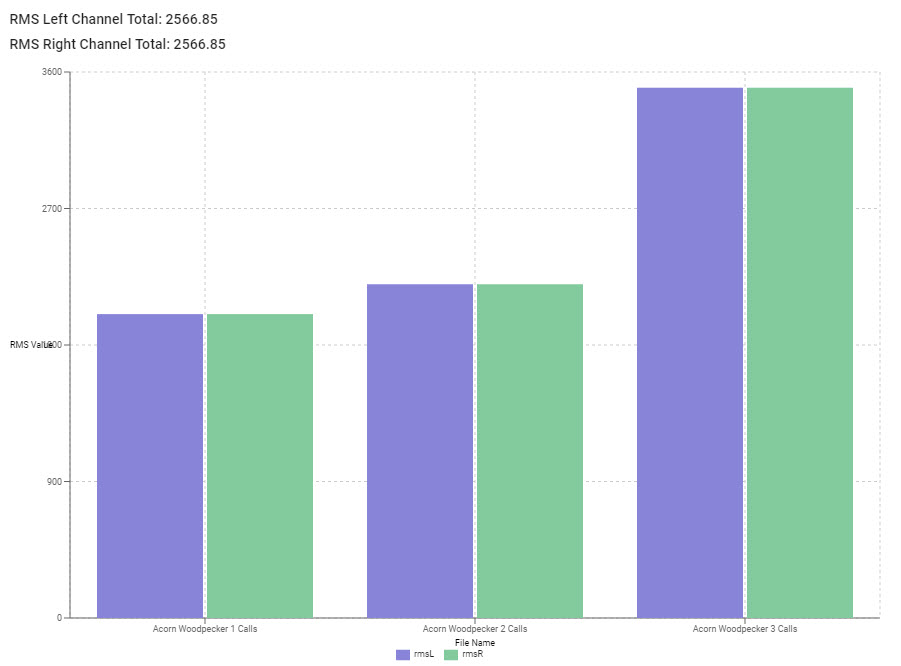
\includegraphics[width=\textwidth]{RMSgraph1} \\[12pt]
\end{center}
As RMS is a single value output, it is best to just display those values for each channel, and use a simple bar chart to represent them visually.
